\documentclass[12pt,twoside]{article}

\textwidth 17cm \textheight 25cm \evensidemargin 0cm
\oddsidemargin 0cm \topmargin -2cm
\parindent 0pt
%\parskip \bigskipamount

\usepackage{graphicx}
\usepackage[dutch]{babel}
\usepackage{amssymb,amsthm,amsmath}
%\usepackage{dot2texi}
\usepackage[utf8]{inputenc}
\usepackage{nopageno}
\usepackage{pdfpages}
\usepackage{enumerate}
\usepackage{caption}
\usepackage{wrapfig}
\usepackage{pgf,tikz,pgfplots}
\pgfplotsset{compat=1.15}
\usepackage{color}
\usetikzlibrary{arrows}
\usetikzlibrary{patterns}
\usepackage{fancyhdr}
\pagestyle{fancy}
\usepackage[version=3]{mhchem}
\usepackage{multicol}
\usepackage{fix-cm}
\usepackage{setspace}
\usepackage{mhchem}
\usepackage{xhfill}
\usepackage{parskip}
\usepackage{cancel}
\usepackage{mdframed}
\usepackage{url}
\usepackage{mathtools}
\usepackage{changepage}

\newcommand{\todo}[1]{{\color{red} TODO: #1}}

\newcommand{\degree}{\ensuremath{^\circ}}
\newcommand\rad{\qopname\relax o{\mathrm{rad}}}

\newcommand\ggd{\qopname\relax o{\mathrm{ggd}}}

\pgfmathdeclarefunction{gauss}{2}{%
  \pgfmathparse{1/(#2*sqrt(2*pi))*exp(-((x-#1)^2)/(2*#2^2))}%
}

\def\LRA{\Leftrightarrow}

\newcommand{\zrmbox}{\framebox{\phantom{EXE}}\phantom{X}}
\newcommand{\zrm}[1]{\framebox{#1}}

% environment oefening:
% houdt een teller bij die de oefeningen nummert, probeert ook de oefening op één pagina te houden
\newcounter{noefening}
\setcounter{noefening}{0}
\newenvironment{oefening}
{
  \stepcounter{noefening}
  \pagebreak[0]
  \begin{minipage}{\textwidth}
  \vspace*{0.7cm}{\large\bf Oefening \arabic{noefening}}
}{%
  \end{minipage}
}

\usepackage{calc}

% vraag
\reversemarginpar
\newcounter{punten}
\setcounter{punten}{0}
\newcounter{nvraag}
\setcounter{nvraag}{1}
\newlength{\puntwidth}
\newlength{\boxwidth}
\newcommand{\vraag}[1]{
\settowidth{\puntwidth}{\Large{#1}}
\setlength{\boxwidth}{1.5cm}
\addtolength{\boxwidth}{-\puntwidth}
{\large\bf Vraag \arabic{nvraag} \addtocounter{nvraag}{1}}\vspace*{-0.5cm}
{\marginpar{\color{lightgray}\fbox{\parbox{1.5cm}{\vspace*{1cm}\hspace*{\boxwidth}{\Large{#1}}}}}
\vspace*{0.5cm}}
\addtocounter{punten}{#1}}

% arulefill
\def\arulefill{\leavevmode{\xrfill[-5pt]{0.3pt}[lightgray]\endgraf}\vspace*{0.2cm}}

% \arules{n}
\newcommand{\arules}[1]{
\color{lightgray}
%\vspace*{0.05cm}
\foreach \n in {1,...,#1}{
  \vspace*{0.75cm}
  \hrule height 0.3pt\hfill
}\color{black}\vspace*{0.2cm}}

% \arule{x}
\newcommand{\arule}[1]{
\color{lightgray}{\raisebox{-0.1cm}{\rule[-0.05cm]{#1}{0.3pt}}}\color{black}
}

% \abox{y}
\newcommand{\abox}[1]{
\fbox{
\begin{minipage}{\textwidth- 4\fboxsep}
\hspace*{\textwidth}\vspace{#1}
\end{minipage}
}
}

\newcommand{\ruitjes}[1]{
\definecolor{cqcqcq}{rgb}{0.85,0.85,0.85}
\hspace*{-2.5cm}
\begin{tikzpicture}[scale=1.04,line cap=round,line join=round,>=triangle 45,x=1.0cm,y=1.0cm]
\draw [color=cqcqcq, xstep=0.5cm, ystep=0.5cm] (0,-#1) grid (20.5,0);
\end{tikzpicture}
}


\newcommand{\assenstelsel}[5][1]{
\definecolor{cqcqcq}{rgb}{0.65,0.65,0.65}
\begin{tikzpicture}[line cap=round,line join=round,>=triangle 45,x=#1cm,y=#1cm]
\draw [color=cqcqcq,dash pattern=on 1pt off 1pt, xstep=1.0cm,ystep=1.0cm] (#2,#4) grid (#3,#5);
\draw[->,color=black] (#2,0) -- (#3,0);
%\draw[shift={(1,0)},color=black] (0pt,2pt) -- (0pt,-2pt) node[below] {\footnotesize $1$};
%\draw[color=black] (#3.25,0.07) node [anchor=south west] {$x$};
\draw[->,color=black] (0,#4) -- (0,#5);
%\draw[shift={(0,1)},color=black] (2pt,0pt) -- (-2pt,0pt) node[left] {\footnotesize $1$};
\draw[color=black] (0.09,#5.25) node [anchor=west] {\phantom{$y$}};
%\draw[color=black] (0pt,-10pt) node[right] {\footnotesize $0$};
\end{tikzpicture}
}

\newcommand{\getallenas}[3][1]{
\definecolor{cqcqcq}{rgb}{0.65,0.65,0.65}
\begin{tikzpicture}[scale=#1,line cap=round,line join=round,>=triangle 45,x=1.0cm,y=1.0cm]
\draw [color=cqcqcq,dash pattern=on 1pt off 1pt, xstep=1.0cm,ystep=1.0cm] (#2,-0.2) grid (#3,0.2);
\draw[->,color=black] (#2.25,0) -- (#3.5,0);
\draw[shift={(0,0)},color=black] (0pt,2pt) -- (0pt,-2pt) node[below] {\footnotesize $0$};
\draw[shift={(1,0)},color=black] (0pt,2pt) -- (0pt,-2pt) node[below] {\footnotesize $1$};
\draw[color=black] (#3.25,0.07) node [anchor=south west] {$\mathbb{R}$};
\end{tikzpicture}
}

\newcommand{\visgraad}[1]{\begin{tabular}{p{0.5cm}|p{#1}}&\\\hline\\\end{tabular}}

\newcommand{\tekenschema}[2]{\begin{tabular}{p{0.5cm}|p{#1}}&\\\hline\\[#2]\end{tabular}}

% schema van Horner
\newcommand{\schemahorner}{
\begin{tabular}{p{0.5cm}|p{7cm}}
&\\[1.5cm]
\hline\\
\end{tabular}}

% geef tabular iets meer ruimte
\setlength{\tabcolsep}{14pt}
\renewcommand{\arraystretch}{1.5}

\newcommand{\toets}[3]{
\thispagestyle{plain}
\vspace*{-2.5cm}
\begin{tikzpicture}[remember picture, overlay]
    \node [shift={(15.25 cm,-1.6cm)}] {%
        \includegraphics[width=1.8cm]{/home/ppareit/kaa1415/logokaavelgem.png}%
    };%
\end{tikzpicture}

\begin{tabular}{|llc|c|}
\hline
\vspace*{-0.5cm}
&&&\\
Naam & \arule{4cm} & {\Large\bf KA AVELGEM} & \\
\vspace*{-0.75cm}
&&&\\
Klas & \arule{4cm} & {\Large\bf 20...-...-...} & \\
\hline
\vspace*{-0.75cm}
&&&\\
Toets & {\bf #2} & {\large\bf #1} & Beoordeling\\
\vspace*{-0.75cm}
&&&\\
Onderwerp & \multicolumn{2}{l|}{\bf #3} &\\
\hline
\end{tabular}
}

\newcommand{\oefeningen}[1]{

\fancyhead[LE, RO]{\vspace{0.5cm} #1}
%\thispagestyle{plain}

{\bf \Large \centering Oefeningen: #1}

}

\raggedbottom

\newcommand\vl{\qopname\relax o{\mathrm{vl}}}

\newcommand\dom{\qopname\relax o{\mathrm{dom}}}
\newcommand\ber{\qopname\relax o{\mathrm{ber}}}

\newcommand\mC{\qopname\relax o{\mathrm{mC}}}
\newcommand\uC{\qopname\relax o{\mathrm{{\mu}C}}}
\newcommand\C{\qopname\relax o{\mathrm{C}}}

\newcommand\W{\qopname\relax o{\mathrm{W}}}
\newcommand\kW{\qopname\relax o{\mathrm{kW}}}
\newcommand\kWh{\qopname\relax o{\mathrm{kWh}}}


\newcommand\V{\qopname\relax o{\mathrm{V}}}
\newcommand\ohm{\qopname\relax o{\mathrm{\Omega}}}
\newcommand\kohm{\qopname\relax o{\mathrm{k\Omega}}}


\newcommand\N{\qopname\relax o{\mathrm{N}}}

\newcommand\Nperkg{\qopname\relax o{\mathrm{N/kg}}}

\newcommand\Nperm{\qopname\relax o{\mathrm{N/m}}}

\newcommand\gpermol{\qopname\relax o{\mathrm{g/mol}}}


\newcommand\kgperm{\qopname\relax o{\mathrm{kg/m}}}
\newcommand\kgperdm{\qopname\relax o{\mathrm{kg/dm}}}
\newcommand\gpercm{\qopname\relax o{\mathrm{g/cm}}}
\newcommand\gperml{\qopname\relax o{\mathrm{g/ml}}}


\newcommand{\mA}{\;\mbox{mA}}
\newcommand{\A}{\;\mbox{A}}
\newcommand{\MA}{\;\mbox{MA}}

\newcommand{\us}{\;\mu\mbox{s}}
\newcommand\s{\qopname\relax o{\mathrm{s}}}

\newcommand\h{\qopname\relax o{\mathrm{h}}}

\newcommand{\kmperh}{\;\mbox{km/h}}
\newcommand{\mpers}{\;\mbox{m/s}}
\newcommand{\kmpermin}{\;\mbox{km/min}}
\newcommand{\kmpers}{\;\mbox{km/s}}

\newcommand{\mph}{\;\mbox{mph}}

\newcommand{\Hz}{\;\mbox{Hz}}

\newcommand\Gm{\qopname\relax o{\mathrm{Gm}}}
\newcommand\Mm{\qopname\relax o{\mathrm{Mm}}}
\newcommand\km{\qopname\relax o{\mathrm{km}}}
\newcommand\hm{\qopname\relax o{\mathrm{hm}}}
\newcommand\dam{\qopname\relax o{\mathrm{dam}}}
\newcommand\m{\qopname\relax o{\mathrm{m}}}
\newcommand\dm{\qopname\relax o{\mathrm{dm}}}
\newcommand\cm{\qopname\relax o{\mathrm{cm}}}
\newcommand\mm{\qopname\relax o{\mathrm{mm}}}
\newcommand\um{\qopname\relax o{\mathrm{{\mu}m}}}
\newcommand\nm{\qopname\relax o{\mathrm{nm}}}


\newcommand\Gg{\qopname\relax o{\mathrm{Gg}}}
\newcommand\Mg{\qopname\relax o{\mathrm{Mg}}}
\newcommand\kg{\qopname\relax o{\mathrm{kg}}}
\newcommand\hg{\qopname\relax o{\mathrm{hg}}}
\renewcommand\dag{\qopname\relax o{\mathrm{dag}}}
\newcommand\g{\qopname\relax o{\mathrm{g}}}
\newcommand\dg{\qopname\relax o{\mathrm{dg}}}
\newcommand\cg{\qopname\relax o{\mathrm{cg}}}
\newcommand\mg{\qopname\relax o{\mathrm{mg}}}
\newcommand\ug{\qopname\relax o{\mathrm{{\mu}g}}}
\renewcommand\ng{\qopname\relax o{\mathrm{ng}}}

\newcommand\ton{\qopname\relax o{\mathrm{ton}}}

\newcommand\Gl{\qopname\relax o{\mathrm{Gl}}}
\newcommand\Ml{\qopname\relax o{\mathrm{Ml}}}
\newcommand\kl{\qopname\relax o{\mathrm{kl}}}
\newcommand\hl{\qopname\relax o{\mathrm{hl}}}
\newcommand\dal{\qopname\relax o{\mathrm{dal}}}
\renewcommand\l{\qopname\relax o{\mathrm{l}}}
\newcommand\dl{\qopname\relax o{\mathrm{dl}}}
\newcommand\cl{\qopname\relax o{\mathrm{cl}}}
\newcommand\ml{\qopname\relax o{\mathrm{ml}}}
\newcommand\ul{\qopname\relax o{\mathrm{{\mu}l}}}
\newcommand\nl{\qopname\relax o{\mathrm{nl}}}

\newcommand\MJ{\qopname\relax o{\mathrm{MJ}}}
\newcommand\kJ{\qopname\relax o{\mathrm{kJ}}}
\newcommand\J{\qopname\relax o{\mathrm{J}}}

\newcommand\T{\qopname\relax o{\mathrm{T}}}
\newcommand\uT{\qopname\relax o{\mathrm{{\mu}T}}}

\newcommand\grC{\qopname\relax o{\mathrm{{\degree}C}}}

\newcommand\K{\qopname\relax o{\mathrm{K}}}
\newcommand\calperK{\qopname\relax o{\mathrm{cal/K}}}

\newcommand\hPa{\qopname\relax o{\mathrm{hPa}}}
\newcommand\Pa{\qopname\relax o{\mathrm{Pa}}}

\newcommand\dB{\qopname\relax o{\mathrm{dB}}}

\newcommand\Var{\qopname\relax o{\mathrm{Var}}}

\newcommand{\EE}[1]{\cdot 10^{#1}}

\onehalfspacing

%\setlength{\headsep}{0cm}

\newenvironment{exlist}[1] %
{ \begin{multicols}{#1}
  \begin{enumerate}[(a)]
    \setlength{\itemsep}{0.5em} }
{ \end{enumerate}
  \end{multicols} }




\usepackage{versions}
\excludeversion{theorie}
% \includeversion{theorie}

\begin{document}

\pagestyle{fancy}
\lhead{}
\rhead{Oefeningen Matrices en Stelsels}

\begin{theorie}

  \thispagestyle{empty}
  \begin{center}
    \begin{mdframed}
      \centering
      \fontsize{40}{60}\selectfont Matrices en Stelsels
    \end{mdframed}
    \vfill
    \vfill
  \end{center}

  \subsection*{Doelstellingen}
  \vspace*{-0.8cm}
  {\singlespacing
    Je \hfill  {\scriptsize(LP2006-059, LI1.9, ET32,14,31)}
    \begin{itemize}
    \itemsep-0.2em
    \item kent de definitie van een matrix
    \item kent een rijmatrix, een kolommatrix, een vierkante matrix, een driehoeksmatrix, een diagonaalmatrix, de eenheidsmatrix, de nulmatrix
    \item kan matrices optellen, vermenigvuldigen met een reëel getal en vermenigvuldigen
    \item kan matrices transponeren
    \item kan met behulp van ICT vraagstukken oplossen die aanleiding geven tot een migratiematrix of een Lesliematrix
    \item kan van een gegeven stelsel van vergelijkingen van de eerste graad de bijhorende coëfficiëntenmatrix en verhoogde matrix bepalen
    \item kan elementaire rijoperaties toepassen die de gelijkwaardigheid van de overeenstemmende stelsels van vergelijkingen van de eerste graad bewaren
    \item kan de oplossingsmethode van Gauss-Jordan toepassen
    \item kan vraagstukken oplossen die aanleiding geven tot een stelsel van vergelijkingen van de eerste graad
    \end{itemize}}

  \thispagestyle{empty}
  \mbox{}
  \newpage
  \clearpage
  \thispagestyle{empty}
  % \mbox{}
  \tableofcontents
  \newpage
  \clearpage
  \pagenumbering{arabic}

  \fancyhead[RO,LE]{Matrices en Stelsels}
  \fancyhead[RE,LO]{}

\end{theorie}

\section{Definitie}

\begin{oefening}
Gegeven
$$A=\begin{pmatrix}
5 & 4 & 3\\
4 & 3 & 2\\
\end{pmatrix}$$
Bepaal
\begin{enumerate}[(a)]
  \item aantal rijen
  \item aantal kolommen
\end{enumerate}
\end{oefening}

\begin{oefening}
Gegeven
$$A=\begin{pmatrix}
12 & 3.5 & 95\\
4  & 6.3 & 13\\
45 & 2.5 & 22\\
91 & 6.6 & 63\\
\end{pmatrix}$$
Bepaal
\begin{enumerate}[(a)]
  \item $a_{13} \qquad a_{31} \qquad a_{43}$
  \item waar staat $13$ in de matrix $A$
\end{enumerate}
\end{oefening}

\begin{oefening}
De Vlaamse Ruit behelst een stedelijk kerngebied in Vlaanderen rond de grootstedelijke gebieden van Brussel, Gent, Antwerpen en Leuven. Het gebied wordt ook wel Vlaamse diamant of Vlaamse driehoek genoemd.\\
\begin{minipage}{0.5\textwidth}
\begin{enumerate}[(a)]
  \item Gebruik een routeplanner om de afstanden tussen Brussel (B), Gent (G), Antwerpen (A) en Leuven (L) te bepalen.
  \item Maak nu een $4 \times 4$-matrix die de \verb#VAN# en \verb#NAAR# afstanden tussen de verschillende steden weergeeft.
\end{enumerate}
$$\begin{pmatrix}
  B\to B & G\to B & A\to B & L\to B\\
  B\to G & G\to G & A\to G & L\to G\\
  B\to A & G\to A & A\to A & L\to A\\
  B\to L & G\to L & A\to L & L\to L\\
\end{pmatrix}$$
\end{minipage}
\begin{minipage}{0.5\textwidth}
\begin{center}
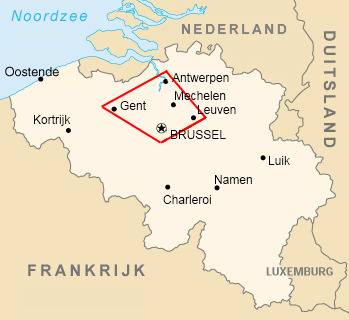
\includegraphics[width=0.99\textwidth]{Vlaamse_ruit}
\end{center}
\end{minipage}
\end{oefening}


\pagebreak

\section{Bijzondere matrices}

\begin{oefening}
Beschouw de matrices
$$
A=\begin{pmatrix}
  -1 & 0\\
  2 & 3\\
  -2 & 1\\
  4 & -3
\end{pmatrix}
\qquad
B=\begin{pmatrix}
  -1 & 0 & 0\\
  2 & -1 & 0\\
  -2 & 1 & -1\\
\end{pmatrix}
\qquad
C=\begin{pmatrix}
  2 & 0\\
  0 & 2\\
\end{pmatrix}
\qquad
D=\begin{pmatrix}
  1
\end{pmatrix}
$$
Zeg telkens welke matrix het is en duid aan tot welke groep van bijzondere matrices ze behoort:
\begin{center}
\begin{tabular}{l|c|c|c|c}
 & A & B & C & D\\
\hline
Grootte $m\times n$ & \arule{2cm} & \arule{2cm} & \arule{2cm} & \arule{2cm} \\  
Nulmatrix & \arule{1cm} & \arule{1cm} & \arule{1cm} & \arule{1cm} \\  
Rijmatrix & \arule{1cm} & \arule{1cm} & \arule{1cm} & \arule{1cm} \\  
Kolommatrix & \arule{1cm} & \arule{1cm} & \arule{1cm} & \arule{1cm} \\  
Vierkante matrix & \arule{1cm} & \arule{1cm} & \arule{1cm} & \arule{1cm} \\  
Diagonaalmatrix & \arule{1cm} & \arule{1cm} & \arule{1cm} & \arule{1cm} \\  
Scalaire matrix & \arule{1cm} & \arule{1cm} & \arule{1cm} & \arule{1cm} \\  
Eenheidsmatrix & \arule{1cm} & \arule{1cm} & \arule{1cm} & \arule{1cm} \\  
Driehoeksmatrix & \arule{1cm} & \arule{1cm} & \arule{1cm} & \arule{1cm} \\  
\end{tabular}
\end{center}
\end{oefening}

\pagebreak
\section{Bewerkingen met matrices}

\begin{oefening}\\
Gegeven:
$$
\scriptsize
A=\begin{pmatrix}
  -1 & 0\\
  2 & 3\\
  -2 & 1\\
  4 & -3
\end{pmatrix}
\quad
B=\begin{pmatrix}
  -2 & 3\\
  1 & -4\\
\end{pmatrix}
\quad
C=\begin{pmatrix}
  2 & -1 & 0 & 3\\
  1 & 0 & 4 & -1\\
  -2 & -3 & 1 & 0\\
\end{pmatrix}
\quad
D=\begin{pmatrix}
  -3 & 1 & 0 & 4\\
  2 & -2 & 3 & 1\\
  -1 & 2 & 4 & -3\\
  2 & 0 & -1 & 3\\
\end{pmatrix}
\quad
E=\begin{pmatrix}
  -1\\
  0\\
  2\\
\end{pmatrix}
$$
Bereken:
\begin{multicols}{2}
  \begin{enumerate}[(a)]
    \itemsep1em
    \item $(C\cdot D)^T=$
    \item $(D\cdot C^T\cdot E)^T=$
    \item $2D\cdot A=$
    \item $D^2\cdot C^T=$
    \item $(E^T\cdot C\cdot A)^T=$
    \item $E\cdot D - 2C=$
    \item $B^2\cdot A^T\cdot D=$
    \item $A^T\cdot C^T\cdot E=$
    \item $3B\cdot A^T=$
    \item $E^T\cdot(-C)\cdot 2A=$
  \end{enumerate}
\end{multicols}
\end{oefening}

\begin{oefening}\\
Gegeven:
$$
\scriptsize
A=\begin{pmatrix}
  0 & 3\\
  -2 & -1\\
  2 & 1\\
  3 & -4
\end{pmatrix}
\quad
B=\begin{pmatrix}
  -4 & -3\\
  1 & 0\\
\end{pmatrix}
\quad
C=\begin{pmatrix}
  -2 & 1 & -2 & 0\\
  3 & -1 & -4 & 0\\
  2 & 0 & -1 & -3\\
\end{pmatrix}
\quad
D=\begin{pmatrix}
  1 & -1 & 3 & 0\\
  3 & 2 & 2 & 4\\
  -3 & -4 & 2 & 1\\
  0 & 2 & 1 & -3\\
\end{pmatrix}
\quad
E=\begin{pmatrix}
  0\\
  -2\\
  1\\
\end{pmatrix}
$$
Bereken:
\begin{multicols}{2}
  \begin{enumerate}[(a)]
    \itemsep1em
    \item $(C\cdot D)^T=$
    \item $(D\cdot C^T\cdot E)^T=$
    \item $2D\cdot A=$
    \item $D^2\cdot C^T=$
    \item $(E^T\cdot C\cdot A)^T=$
    \item $E\cdot D - 2C=$
    \item $B^2\cdot A^T\cdot D=$
    \item $A^T\cdot C^T\cdot E=$
    \item $3B\cdot A^T=$
    \item $E^T\cdot(-C)\cdot 2A=$
  \end{enumerate}
\end{multicols}
\end{oefening}

\pagebreak
\section{Migratie- en Lesliematrices}


\begin{oefening}
In een ontwikkelingsland is er een wekelijks mededelingsprogramma voor landbouwers waarin een technologische evolutie wordt uiteengezet. Deze landbouwers hebben onderling geen contact. De kans dat een landbouwer luistert is $20$ \%. We gaan ervan uit dat in het ontwikkelingsland met 250 duizend landbouwers er initieel geen enkele landbouwer iets van de innovaties weet.

\begin{enumerate}[(a)]
  \item Stel de gegevens grafisch voor met behulp van een graaf.
  \item Stel een migratie matrix op.
  \item Hoeveel landbouwers zullen na één maand op de hoogte zijn van de technologische vooruitgang?
\end{enumerate}
\end{oefening}

\pagebreak
\section{Gauss-Jordan}

\begin{oefening}
Los op in $\mathbb{R}^3$:
\begin{multicols}{2}
\begin{enumerate}[(a)]
  \item$$\left\{
\begin{aligned}
  x + 2y -z &= -4\\
  2x+3y+z   &= 3\\
  5x-y+3z   &= 1
\end{aligned}\right.$$
  \item$$\left\{
\begin{aligned}
  -3x -7y +6z &= 6\\
  x+3y-2z   &= 0\\
  2x+y+4z   &= 25
\end{aligned}\right.$$
  \item$$\left\{
\begin{aligned}
  3x +2y +4z &= -4\\
  x+y+z   &= 1\\
  5x-4y+3z   &= -3
\end{aligned}\right.$$
  \item$$\left\{
\begin{aligned}
  3x -4y +z &= 35\\
  x-y+2z   &= 11\\
  -5x+2y-2z   &= -26
\end{aligned}\right.$$
  \item$$\left\{
\begin{aligned}
  x -y + 2z &= -1\\
  4x-3y+5z   &= 18\\
  -x+y+4z   &= -5
\end{aligned}\right.$$
\end{enumerate}
\end{multicols}
\end{oefening}

\begin{oefening}
Los op in $\mathbb{R}^3$:
\begin{multicols}{2}
\begin{enumerate}[(a)]
  \item$$\left\{
    \begin{aligned}
      3x - 7y + 2z &= 2\\
      -x + 3y      &= -2\\
      x  - 2y +  z &= 0
    \end{aligned}\right.$$
  \item$$\left\{
    \begin{aligned}
        x - 3y -  z &= 2\\
      -2x + 5y + 3z &= 4\\
       4x -11y - 5z &= 5
    \end{aligned}\right.$$
  \item$$\left\{
    \begin{aligned}
      2x + 3y + 5z &= 9\\
       x + 2y + 3z &= 4\\
       x +  z &= 5
    \end{aligned}\right.$$
  \item$$\left\{
    \begin{aligned}
      2x +  y - 2z &= -2\\
      3x + 2y -  z &=  4\\
       x +  y +  z &=  6
    \end{aligned}\right.$$
  \item$$\left\{
    \begin{aligned}
       x + 2y +  z &= 3\\
      2x + 3y + 4z &= 5\\
      4x + 7y + 6z &= 9
    \end{aligned}\right.$$
\end{enumerate}
\end{multicols}
\end{oefening}

\begin{oefening}
Los op in $\mathbb{R}^3$:
\begin{multicols}{2}
\begin{enumerate}[(a)]
  \item$$\left\{
    \begin{aligned}
      3x -  y +  z &= 29\\
      x  + 3y +30z &=  6\\
      x  -  y +  z &= 17
    \end{aligned}\right.$$
  \item$$\left\{
    \begin{aligned}
      -2x + 4y - 6z &= -46\\
       3x +  y + 38 &= 4z\\
      -4x - 5y + 2z &= 56
    \end{aligned}\right.$$
  \item$$\left\{
    \begin{aligned}
       y - 3x - 2z &= -17\\
      4x +  z - 3y &= 31\\
      2y +  x &= -13 + 4z
    \end{aligned}\right.$$
  \item$$\left\{
    \begin{aligned}
      7z + 3x + 14 &= y\\
       y -  x - 3z &= 4\\
       z - 5x - 3y &= 4
    \end{aligned}\right.$$
  \item$$\left\{
    \begin{aligned}
      2x -  y + 3z &= -4\\
       x + 5z      &= 7\\
      2y +  z + 3x &= 1
    \end{aligned}\right.$$
\end{enumerate}
\end{multicols}
\end{oefening}

\pagebreak

\section{Vraagstukken op stelsels}

\begin{oefening}
In een winkeltje in het dorp kost 200 gram nougat, 300 gram chocolaatjes en 100 gram marsepein 
9 EUR.  Voor 300 gram nougat, 100 gram chocolaatjes en 400 gram marsepein betaal je 12,7 EUR.
Hoeveel kost 200 gram nougat, 200 gram chocolaatjes en 200 gram marsepein als je weet dat
1 kg chocolaatjes 5 euro minder kost dan 1 kg nougat?
\end{oefening}

\begin{oefening}
Boer Moors kweekt geiten, schapen en struisvogels.  Toen ik hem vroeg hoeveel stuks hij van elke soort had, kreeg ik het volgende antwoord.\\
“Wanneer één derde van mijn geiten schapen zou zijn, had ik evenveel geiten als schapen en struisvogels samen.  
Wanneer één derde van mijn schapen struisvogels zou zijn, had ik vijfmaal zoveel geiten als struisvogels.
Wanneer één derde van mijn struisvogels geiten zou zijn, had ik 470 geiten.”\\
Kan jij achterhalen hoeveel geiten, schapen en struisvogels boer Moors heeft?
\end{oefening}

\begin{oefening}
“Hoe oud ben je?” vraagt een jongen aan een meisje.
“Wel”, zegt ze, “mijn mama en ik zijn samen 56 jaar.  Mijn oma en ik zijn samen 80 jaar en mijn mama en mijn oma zijn samen 100 jaar.”
Hoe oud zijn het meisje, haar mama en haar oma?
\end{oefening}

\begin{oefening}
Anke, Bert en Chris willen een geschenk kopen voor het huwelijk van een vriend en vriendin.
Ze overlopen samen hoeveel geld ze hebben.
Anke en Bert hebben samen 20 euro meer dan Chris.
Bert en Chris hebben samen 32 euro meer dan Anke.
Anke en Chris hebben samen 28 euro meer dan Bert.
Hoeveel heeft ieder nog in zijn portemonnee?
\end{oefening}

\begin{oefening}
Anna, Brigitte en Charlotte vormen een driegeslacht.  Samen zijn ze 105 jaar oud.  Anna is negen jaar ouder dan Brigitte en Charlotte samen.  Jammer genoeg komen Anna en Charlotte samen nog drie jaartjes tekort om dubbel zo oud te zijn als Brigitte.
Hoe oud zijn deze drie dames?
\end{oefening}

\begin{oefening}
Bepaal de vergelijking $y=ax^2+bx+c$ van de parabool die door de punten $(1,1)$, $(-1, 5)$ en $(2,2)$ gaat.
\end{oefening}

\begin{oefening}
Bepaal een natuurlijk getal bestaande uit drie cijfers. Het cijfer van de tientallen is het gemiddelde van het cijfer van de honderdtallen en het cijfer van de eenheden. Telt men 396 op bij het getal, dan bekomt men een getal met dezelfde cijfers als het gevraagde getal maar in omgekeerde volgorde. Deelt men het getal door de som van de cijfers, dan is het quotiënt 26 en de rest 0.
\end{oefening}

\begin{oefening}
Een melkveehoudersbedrijf wenst een aantal tankwagens te kopen om zelf de melk te transporteren. Ze kunnen 24 tankwagens kopen en in het totaal moeten ze daarmee 250000 liter melk vervoeren. Er zijn drie types tankwagens aanwezig, tankwagens met een inhoud van 6000, van 8000 en van 18000 liter. Hoeveel tankwagens van elk type zijn nodig.
\end{oefening}

\begin{oefening}
Bepaal het functievoorschrift van een veeltermfunctie $f$ van de derde graad waarvoor $-1$ en $2$ nulwaarden zijn en waarvoor geldt:
$$f(1)=f(-2)=-4$$
\end{oefening}

\begin{oefening}
Bepaal het functievoorschrift van een monische derdegraadsfunctie $f$ die als nulwaarde $1$ en $2$ heeft en waarvoor $(5,120)\in f$ is.
\end{oefening}

\begin{oefening}
Een cirkel gaat door de punten $(2,-2)$, $(-1, -3)$ en $(-2,8)$. Geef de vergelijking van de cirkel.
\end{oefening}

\begin{oefening}
Een diëtist in een ziekenhuis moet een speciaal dieet samenstellen bestaande uit drie ingrediënten. Het dieet moet juist 340 eenheden calcium, 180 eenheden ijzer en 220 eenheden vitamine A bevatten. Het aantal eenheden per $30$ gram van de drie ingrediënten wordt gegeven door de volgende tabel:
\begin{center}
  \begin{tabular}{lccc}
               &\multicolumn{3}{c}{Eenheden per 30 gram}\\
    \hline
               & ingrediënt A & ingrediënt B & ingrediënt C\\
    \hline
    Calcium    & 30           & 10           & 20\\
    Iron       & 10           & 10           & 20\\
    Vitamine A & 10           & 30           & 20\\
  \end{tabular}
\end{center}
\begin{enumerate}[(a)]
  \item Hoeveel gram van elk ingrediënt moet gebruikt worden om te voldoen aan het dieet?
  \item Hoe wordt het dieet beïnvloed als we ingrediënt C niet mogen gebruiken?
  \item Hoe wordt het dieet beïnvloed als we niet langer moeten voldoen aan de vitamine A vereiste?
\end{enumerate}
\end{oefening}


\end{document}


